\documentclass[10pt]{article}

%%%%%%%%%%%%%%%%%%%%%%%%%%%%%%%%%%%%%%%%%%%%%%%%%%%%%%%%%%%%%%%%%%%%%%%%%%%%%%%%
% LaTeX Imports
%%%%%%%%%%%%%%%%%%%%%%%%%%%%%%%%%%%%%%%%%%%%%%%%%%%%%%%%%%%%%%%%%%%%%%%%%%%%%%%%
\usepackage{amsfonts}                                                   % Math fonts
\usepackage{amsmath}                                                    % Math formatting
\usepackage{amssymb}                                                    % Math formatting
\usepackage{amsthm}                                                     % Math Theorems
\usepackage{arydshln}                                                   % Dashed hlines
\usepackage{attachfile}                                                 % AttachFiles
\usepackage{cancel}                                                     % Cancelled math
\usepackage{caption}                                                    % Figure captioning
\usepackage{color}                                                      % Nice Colors
\input{./lib/dragon.inp}                                                % Tikz dragon curve
\usepackage[ampersand]{easylist}                                        % Easy lists
\usepackage{fancyhdr}                                                   % Fancy Header
\usepackage[T1]{fontenc}                                                % Specific font-encoding
%\usepackage[margin=1in, marginparwidth=2cm, marginparsep=2cm]{geometry} % Margins
\usepackage{graphicx}                                                   % Include images
\usepackage{hyperref}                                                   % Referencing
\usepackage[none]{hyphenat}                                             % Don't allow hyphenation
\usepackage{lipsum}                                                     % Lorem Ipsum Dummy Text
\usepackage{listings}                                                   % Code display
\usepackage{marginnote}                                                 % Notes in the margin
\usepackage{microtype}                                                  % Niceness
\usepackage{lib/minted}                                                 % Code display
\usepackage{multirow}                                                   % Multirow tables
\usepackage{pdfpages}                                                   % Include pdfs
\usepackage{pgfplots}                                                   % Create Pictures
\usepackage{rotating}                                                   % Figure rotation
\usepackage{setspace}                                                   % Allow double spacing
\usepackage{subcaption}                                                 % Figure captioning
\usepackage{tikz}                                                       % Create Pictures
\usepackage{tocloft}                                                    % List of Equations
%%%%%%%%%%%%%%%%%%%%%%%%%%%%%%%%%%%%%%%%%%%%%%%%%%%%%%%%%%%%%%%%%%%%%%%%%%%%%%%%
% Package Setup
%%%%%%%%%%%%%%%%%%%%%%%%%%%%%%%%%%%%%%%%%%%%%%%%%%%%%%%%%%%%%%%%%%%%%%%%%%%%%%%%
\hypersetup{%                                                           % Setup linking
    colorlinks=true,
    linkcolor=black,
    citecolor=black,
    filecolor=black,
    urlcolor=black,
}
\RequirePackage[l2tabu, orthodox]{nag}                                  % Nag about bad syntax
\renewcommand*\thesection{\arabic{section} }                             % Reset numbering
\renewcommand{\theFancyVerbLine}{ {\arabic{FancyVerbLine} } }              % Needed for code display
\renewcommand{\footrulewidth}{0.4pt}                                    % Footer hline
\setcounter{secnumdepth}{3}                                             % Include subsubsections in numbering
\setcounter{tocdepth}{3}                                                % Include subsubsections in toc
%%%%%%%%%%%%%%%%%%%%%%%%%%%%%%%%%%%%%%%%%%%%%%%%%%%%%%%%%%%%%%%%%%%%%%%%%%%%%%%%
% Custom commands
%%%%%%%%%%%%%%%%%%%%%%%%%%%%%%%%%%%%%%%%%%%%%%%%%%%%%%%%%%%%%%%%%%%%%%%%%%%%%%%%
\newcommand{\nvec}[1]{\left\langle #1 \right\rangle}                    %  Easy to use vector
\newcommand{\ma}[0]{\mathbf{A} }                                         %  Easy to use vector
\newcommand{\mb}[0]{\mathbf{B} }                                         %  Easy to use vector
\newcommand{\abs}[1]{\left\lvert #1 \right\rvert}                       %  Easy to use abs
\newcommand{\pren}[1]{\left( #1 \right)}                                %  Big parens
\let\oldvec\vec
\renewcommand{\vec}[1]{\oldvec{\mathbf{#1} } }                            %  Vector Styling
\newtheorem{thm}{Theorem}                                               %  Define the theorem name
\newtheorem{definition}{Definition}                                     %  Define the definition name
\definecolor{bg}{rgb}{0.95,0.95,0.95}
\newcommand{\java}[4]{\vspace{10pt}\inputminted[firstline=#2,
                                 lastline=#3,
                                 firstnumber=#2,
                                 gobble=#4,
                                 frame=single,
                                 label=#1,
                                 bgcolor=bg,
                                 linenos]{java}{#1} }
\newcommand{\python}[4]{\vspace{10pt}\inputminted[firstline=#2,
                                 lastline=#3,
                                 firstnumber=#2,
                                 gobble=#4,
                                 frame=single,
                                 label=#1,
                                 bgcolor=bg,
                                 linenos]{python}{#1} }
\newcommand{\js}[4]{\vspace{10pt}\inputminted[firstline=#2,
                                 lastline=#3,
                                 firstnumber=#2,
                                 gobble=#4,
                                 frame=single,
                                 label=#1,
                                 bgcolor=bg,
                                 linenos]{js}{#1} }
%%%%%%%%%%%%%%%%%%%%%%%%%%%%%%%%%%%%%%%%%%%%%%%%%%%%%%%%%%%%%%%%%%%%%%%%%%%%%%%%
% Beginning of document items - headers, title, toc, etc...
%%%%%%%%%%%%%%%%%%%%%%%%%%%%%%%%%%%%%%%%%%%%%%%%%%%%%%%%%%%%%%%%%%%%%%%%%%%%%%%%
\pagestyle{fancy}                                                       %  Establishes that the headers will be defined
\fancyhead[LE,LO]{Computer Systems Notes}                                  %  Adds header to left
\fancyhead[RE,RO]{Zoe Farmer}                                       %  Adds header to right
\cfoot{ \thepage }
\lfoot{CSCI 2400}
\rfoot{Han}
\title{Computer Systems Notes}
\author{Zoe Farmer}

%%%%%%%%%%%%%%%%%%%%%%%%%%%%%%%%%%%%%%%%%%%%%%%%%%%%%%%%%%%%%%%%%%%%%%%%%%%%%%%%
% Beginning of document items - headers, title, toc, etc...
%%%%%%%%%%%%%%%%%%%%%%%%%%%%%%%%%%%%%%%%%%%%%%%%%%%%%%%%%%%%%%%%%%%%%%%%%%%%%%%%
\pagestyle{fancy}                                                       %  Establishes that the headers will be defined
\fancyhead[LE,LO]{Homework 3}                                  %  Adds header to left
\fancyhead[RE,RO]{Zoe Farmer}                                       %  Adds header to right
\cfoot{\mlptikz[size=0.25in, text=on, textposx=0, textposy=0, textvalue=\thepage, textscale=0.75in]{applejack}}
\lfoot{APPM 4570}
\rfoot{Hagar}
\title{Homework 3}
\author{Zoe Farmer}
%%%%%%%%%%%%%%%%%%%%%%%%%%%%%%%%%%%%%%%%%%%%%%%%%%%%%%%%%%%%%%%%%%%%%%%%%%%%%%%%
% Beginning of document items - headers, title, toc, etc...
%%%%%%%%%%%%%%%%%%%%%%%%%%%%%%%%%%%%%%%%%%%%%%%%%%%%%%%%%%%%%%%%%%%%%%%%%%%%%%%%
\begin{document}

\maketitle

\begin{easylist}[enumerate]
    @ Consider a system of 6 components pictured in Figure~\ref{fig:arrow}.\newline

    \begin{figure}[!ht]
        \centering
        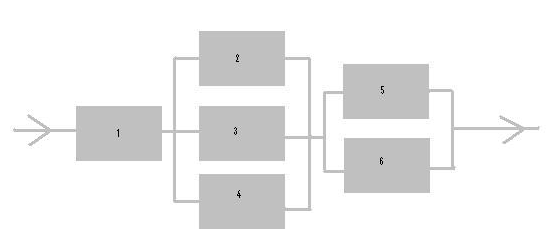
\includegraphics[scale=0.5]{./img/diagram31.png}
        \caption{}
        \label{fig:arrow}
    \end{figure}

    For the system to work, all of the following must be
    satisfied: (1) Component 1 has to work (2) at least one of the components 2, 3, and 4 has to work (3) at least one
    of the components 5 and 6 has to work.\newline

    Component 1 has an exponentially distributed lifetime with a mean of 1/2 year.\newline

    Components 2, 3, and 4 each have an exponentially distributed lifetime with mean lifetime of 1 year. Components 5
    and 6 have exponentially distributed lifetimes with mean lifetime of 1.5 year.

    \begin{table}[!ht]
        \centering
        \begin{tabular}{|l|l|l|}
            \hline
            Component & Lifetime & CDF\\
            \hline
            1 & $(1/2)e^{-(1/2)x}$ & $1 - e^{-(1/2)x}$\\
            \hline
            2 & $e^{-x}$ & $1 - e^{-x}$\\
            \hline
            3 & $e^{-x}$ & $1 - e^{-x}$\\
            \hline
            4 & $e^{-x}$ & $1 - e^{-x}$\\
            \hline
            5 & $(3/2)e^{-(3/2)x}$ & $1 - e^{-(3/2)x}$\\
            \hline
            6 & $(3/2)e^{-(3/2)x}$ & $1 - e^{-(3/2)x}$\\
            \hline
        \end{tabular}
        \caption{Lifetime Distributions}
        \label{table:lifetimes}
    \end{table}

    @@ What is the probability that the system will function uninterruptedly for at least 2 years?
    @@@ We can rephrase this question to ask what's the probability that no piece of the system will fail. This means
    that we're only interested in the probabilities of components 1, 2-4, and 5-6.\newline

    The probability that component 1 will last for at least two years is
    \[
        \int^\infty_2 (1/2)e^{-(1/2)x} \, dx = 0.367879
    \]

    The probability that components 2-3 will last for at least two years is
    \[
        \int^\infty_2 e^{-x} \, dx = 0.135335
    \]

    The probability that components 5-6 will last for at least two years is
    \[
        \int^\infty_2 (3/2)e^{-(3/2)x} \, dx = 0.0497871
    \]

    Any case in which the system remains uninterrupted component 1 must function, therefore we can include its
    probability. Any one of components 2-3 must work, and either 5 or 6. Let $p_i$ be the probability that component $i$
    lasts.

    \[
        \begin{aligned}
            & p_1 \cdot p_2^3 \cdot p_5^2 +\\
            & p_1 \cdot \binom{3}{1} p_2^2 p_2^c \cdot p_5^2 + p_1 \cdot \binom{3}{2} p_2 \cdot {p_2^c}^2 \cdot p_5^2 +\\
            & p_1 \cdot p_2^3 \cdot \binom{2}{1} p_5 \cdot p_5^c +\\
            & p_1 \cdot \binom{3}{1} p_2^2 p_2^c \cdot \binom{2}{1} p_5 \cdot p_5^c +\\
            & p_1 \cdot \binom{3}{2} p_2 \cdot {p_2^c}^2 \cdot \binom{2}{1} p_5 \cdot p_5^c\\
            & = \boxed{0.0126281}
        \end{aligned}
    \]

    @@ What is the probability that the system will fail in the first 3 months of the 2nd year?
    @@@ We can use a derivation of our previous equation, we just need to clarify some terms.\newline

    The probability that component 1 fails in the first 3 months of the 2nd year is
    \[
        \int^{2.25}_2 (1/2)e^{-(1/2)x} \, dx = 0.0813746
    \]

    The probability that components 2-3 fails in the first 3 months of the 2nd year is
    \[
        \int^{2.25}_2 e^{-x} \, dx = 0.0532503
    \]

    The probability that components 5-6 fails in the first 3 months of the 2nd year is
    \[
        \int^{2.25}_2 (3/2)e^{-(3/2)x} \, dx = 0.0262693
    \]

    Using our equation from before with the new probabilities we get $p=\boxed{0.00063876}$.

    @ Let $X$ be a normally distributed random variable with mean 3 and variance 4.
    @@ Let $Y = 5X + 2$. What is the distribution of $Y$? What are its mean and variance?
    @@@ $Y$ will also be normally distributed, however the mean is now calculated by
    \[ E(Y) = E(5X+2) = 5 E(X) + 2 = 17 \]
    The variance similarly changes
    \[ \text{Var}(Y) = \text{Var}(5X+2) = 25 \cdot \text{Var}(x) = 100 \]
    @@ Find $P(Y < 10)$. Find $P(X < 10)$.
    @@@ We can use the definition of a normal distribution to determine the answer.
    \[ p(x;\mu, \sigma^2) = \frac{1}{\sigma\sqrt{2\pi}}\, e^{-\frac{(x - \mu)^2}{2 \sigma^2}} \]
    Now we can define their CDF and find for $x=10$ and get $P(Y < 10) = 0.241964$ and $P(X < 10)=0.999767$
    @@ What is the 99th percentile of the distribution of $Y$?
    @@@ To find this we need to solve for when the cdf of $Y$ equals 0.99. This results in $40.2635$.
    @@ What is the 99th percentile of the distribution of $X$?
    @@@ To find this we need to solve for when the cdf of $X$ equals 0.99. This results in $7.6527$.

    @ Let $X_1$, $X_2$, $X_3$, $X_4$, $X_5$, and $X_6$ denote the numbers of blue, brown, green, orange, red, and yellow
    M\&M candies, respectively, in a sample of size $n$. According to the M\&M website, the color proportions are $p_1 =
    0.24$, $p_2 = 0.13$, $p_3 = 0.16$, $p_4 = 0.20$, $p_5 = 0.13$, and $p_6 = 0.14$.
    @@ If $n = 12$, what is the probability that there are exactly two M\&Ms of each color?
    @@@ Each pair has probability $p_i^2$, and there are $12!$ ways to arrange the pairs, therefore our answer is
    \[ \frac{12!}{2!2!2!2!2!2!} \cdot 0.24^2 \cdot 0.13^2 \cdot 0.16^2 \cdot 0.20^2 \cdot 0.13^2 \cdot 0.14^2 = \boxed{0.00247121} \]
    @@ For $n = 20$, what is the probability that there are at most five orange candies?
    @@@ This can be thought of as a binomial distribution with $p=0.20$. Therefore the probability that there will be at
    most 5 is
    \[
        \begin{aligned}
            & P(0) + P(1) + P(2) + P(3) + P(4) + P(5)\\
            & = \binom{20}{0} {(0.20)}^0 {(0.80)}^{20} + \binom{20}{1} {(0.20)}^1 {(0.80)}^{20} + \cdots + \binom{20}{5} {(0.20)}^5 {(0.80)}^{16}\\
            & = \boxed{0.804208}
        \end{aligned}
    \]
    @@ In a sample of 20 M\&Ms, what is the probability that the total number of candies that are blue, green, or orange
    is at least 10?
    @@@ This is similar to our binomial distribution previously, and can be expressed equivalently as $1 - (P(0) + P(1)
    + \cdots + P(9))$, where we can set $p=0.24+0.16+0.2=0.6$. The probability equals
    \[
        \begin{aligned}
            & 1 - \left( \binom{20}{0} {(0.60)}^0 {(0.40)}^{20} + \binom{20}{1} {(0.58)}^1 {(0.40)}^{19} + \ldots + \binom{20}{9} {(0.58)}^9
            {(0.40)}^{11} \right)\\
            & = \boxed{0.872479}
        \end{aligned}
    \]


    @ Please answer and provide a brief justification of your answer.
    @@ Can covariance between two random variables be less that $-1$?
    @@@ Yes, covariance does not have a range of values, and the covariance between two random variables can be
    virtually anything.
    @@ If covariance between two random variables is negative, does their correlation have to be negative?
    @@@ Yes, a negative covariance indicates a an inverse relationship, and so does a negative correlation.
    @@ If correlation between two random variables is negative, does their covariance have to be negative?
    @@@ Yes, for the same reasons above.
    @@ Can correlation between two random variables be bigger than 1?
    @@@ No. Correlation is limited to $[-1,+1]$, and no values can be larger or smaller.
    @@ If $\text{Cov}(X,Y) = 0.3$, what is $\text{Cov}(100X, Y)$?
    @@@ We can simply pull the constants from the equation and get $\boxed{100 \cdot 0.3 = 30}$.
    @@ If $\text{Corr}(X,Y) = 0.1$, what is $\text{Corr}(100X, Y)$?
    @@@ Multiplying by a positive scalar has no affect on the correlation, therefore we get $\boxed{0.1}$.
    @@ What is $\text{Cov}(X,X)$?
    @@@ The covariance of two of the same random variables is simply the variance, denoted $\sigma^2$.
    @@ What is $\text{Corr}(X,X)$?
    @@@ Since these two random variables are the same, they will have a near perfect linear correlation (assuming enough
    samples are taken) of about 1. If infinite samples are taken than it will be 1.
    @@ What is $\text{Cov}(100X,10X)$?
    @@@ This is equivalent to $1000\sigma^2$.
    @@ What is $\text{Corr}(100X,10X)$?
    @@@ Since both coefficients are positive the correlation remains the same.
    @@ What is $\text{Corr}(X,X^2)$?
    @@@ This has nonlinear correlation, and since we only catch linear correlation this is about zero.

    @ A rock specimen is randomly selected and weighed two different times. Let $w$ denote the true weight (a number) of
    the rock, and let $X_1$ and $X_2$ be the two measured weights. Then $X_1 = w + E_1$, and $X_2 = w + E_2$, where
    $E_1$ and $E_2$ are the two measurement errors. Suppose that $E_1$ and $E_2$ are independent and distributed
    normally with mean 0 and variance equal to $0.1$ (i.e.\ $E_1, E_2 \approx N(0, 0.1)$).
    @@ What is the mean of $X_1$? What is the mean of $X_2$?
    @@@ Similar to our problem above we can split some of these parts up.
    \[
        \begin{aligned}
            E(X_1) = E(w + E_1) = E(E_1) + w = w\\
            E(X_2) = E(w + E_2) = E(E_2) + w = w\\
        \end{aligned}
    \]
    @@ What is $\text{Var}(X_1)$? What is $\text{Var}(X_2)$?
    @@@ Since we are only adding the variance remains the same for both random variables, namely 0.1.
    @@ What is $\text{Corr}(X_1, X_2)$?
    @@@ Since these distributions are independent, the correlation value is approximately 0.
    @@ Implement this problem on your computer using statistical software. How many values of $X_1$ do you need to get
    close to the theoretical values in the previous parts of this problem? How many values of $X_2$ do you need? Paste
    in any code or commands that you used, and be thorough in your answer.
    @@@ When implemented, these trends established in prior answers are not apparent until there are at least 100
    values, and even then it's unclear. In order to get close to our theoretical values, we need to have many many more.
    Setting $n=10,000,000$ shows distinct numbers, however we still aren't very close. In order to have error $\epsilon$
    we'd need to set $n=\infty$ and determine the long-term behavior. If we're more interested in an estimate, the
    trends become somewhat clear after 100 values.

    The code to determine this is below.

    \newpage

\end{easylist}
\end{document}
